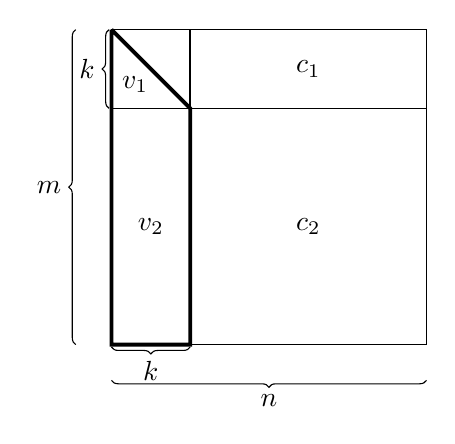
\begin{tikzpicture}
\draw[semithick] (0,0) -- (4,0) -- (4,4)-- (0,4)-- (0,0);


\draw[semithick] (1,0) -- (1,4);
\draw[semithick] (0,3) -- (4,3);
\draw[line width=0.5mm] (0,4) -- (0,0) -- (1,0) -- (1,3) -- (0,4);


\draw[decorate, decoration={brace,mirror}, yshift=-.2ex]  (0,0) -- node[below=0.4ex] {$k$}  (1,0);
\draw[decorate, decoration={brace}, xshift=-.2ex]  (0,3) -- node[left=0.4ex] {$k$}  (0,4);
\draw[decorate, decoration={brace,mirror}, yshift=-3ex]  (0,0) -- node[below=0.4ex] {$n$}  (4,0);
\draw[decorate, decoration={brace}, xshift=-3ex]  (0,0) -- node[left=0.4ex] {$m$}  (0,4);

\draw (0.3,3.3) node {$v_1$};
\draw (0.5,1.5) node {$v_2$};
\draw (2.5,3.5) node {$c_1$};
\draw (2.5,1.5) node {$c_2$};



\end{tikzpicture}